%% Template for Stata-Journal Quarto manuscript

%% Main

% main.tex - a driver for your Stata Journal insert
% This file should only be changed according to the AUTHOR notes below.
% The Stata Press document class

\documentclass[bib]{statapress}

% Page dimensions
\usepackage[crop,newcenter,frame]{pagedims}
% The Stata Journal styles
\usepackage{sj}
% Stata Log listings and useful macros
\usepackage{stata}
% Encapsulated PostScript figures
\usepackage{epsfig}
% Shadow package to render technical note figure
\usepackage{shadow}
\usepackage{amsmath,amssymb} 
% EDITORS: volume number, issue number, month, and year
\usepackage{setspace}
%% Hide Links
%CodeThis is for Executed code. But may not be necessary
\usepackage{color}
\usepackage{fancyvrb}
\newcommand{\VerbBar}{|}
\newcommand{\VERB}{\Verb[commandchars=\\\{\}]}
\DefineVerbatimEnvironment{Highlighting}{Verbatim}{commandchars=\\\{\}}
% Add ',fontsize=\small' for more characters per line
\usepackage{framed}
\definecolor{shadecolor}{RGB}{255,255,255}
\newenvironment{Shaded}{\begin{snugshade}}{\end{snugshade}}
\newcommand{\KeywordTok}[1]{\textcolor[rgb]{0.00,0.0,0.0}{#1}}
\newcommand{\NormalTok}[1]{\textcolor[rgb]{0.00,0.0,0.0}{#1}}




%% Ref

 

\sjsetissue{vv}{ii}{mm}{yyyy}

%%%%%%%%%%%%%%%%%%%%%%%%%%%%%%%%%%%%%%%%%%%%%%%%%%%%%%%%%%%%%%%%%%%%%%%%%%%%%%%


\providecommand{\tightlist}{%
  \setlength{\itemsep}{0pt}\setlength{\parskip}{0pt}}\usepackage{longtable,booktabs,array}
\usepackage{calc} % for calculating minipage widths
% Correct order of tables after \paragraph or \subparagraph
\usepackage{etoolbox}
\makeatletter
\patchcmd\longtable{\par}{\if@noskipsec\mbox{}\fi\par}{}{}
\makeatother
% Allow footnotes in longtable head/foot
\IfFileExists{footnotehyper.sty}{\usepackage{footnotehyper}}{\usepackage{footnote}}
\makesavenoteenv{longtable}
\usepackage{graphicx}
\makeatletter
\def\maxwidth{\ifdim\Gin@nat@width>\linewidth\linewidth\else\Gin@nat@width\fi}
\def\maxheight{\ifdim\Gin@nat@height>\textheight\textheight\else\Gin@nat@height\fi}
\makeatother
% Scale images if necessary, so that they will not overflow the page
% margins by default, and it is still possible to overwrite the defaults
% using explicit options in \includegraphics[width, height, ...]{}
\setkeys{Gin}{width=\maxwidth,height=\maxheight,keepaspectratio}
% Set default figure placement to htbp
\makeatletter
\def\fps@figure{htbp}
\makeatother

\makeatletter
\@ifpackageloaded{caption}{}{\usepackage{caption}}
\AtBeginDocument{%
\ifdefined\contentsname
  \renewcommand*\contentsname{Table of contents}
\else
  \newcommand\contentsname{Table of contents}
\fi
\ifdefined\listfigurename
  \renewcommand*\listfigurename{List of Figures}
\else
  \newcommand\listfigurename{List of Figures}
\fi
\ifdefined\listtablename
  \renewcommand*\listtablename{List of Tables}
\else
  \newcommand\listtablename{List of Tables}
\fi
\ifdefined\figurename
  \renewcommand*\figurename{Figure}
\else
  \newcommand\figurename{Figure}
\fi
\ifdefined\tablename
  \renewcommand*\tablename{Table}
\else
  \newcommand\tablename{Table}
\fi
}
\@ifpackageloaded{float}{}{\usepackage{float}}
\floatstyle{ruled}
\@ifundefined{c@chapter}{\newfloat{codelisting}{h}{lop}}{\newfloat{codelisting}{h}{lop}[chapter]}
\floatname{codelisting}{Listing}
\newcommand*\listoflistings{\listof{codelisting}{List of Listings}}
\makeatother
\makeatletter
\makeatother
\makeatletter
\@ifpackageloaded{caption}{}{\usepackage{caption}}
\@ifpackageloaded{subcaption}{}{\usepackage{subcaption}}
\makeatother
\begin{document}

%% AUTHOR:  Include your article here.

%% TITLE

 
\title[]{Simplifying the Estimation of Correlated Random Effects Models}


\makeatletter

\inserttype[st0001]{article}
\author{}{
Fernando Rios-Avila\\
Levy Economics Institute of Bard College\\Annandale-on-Hudson, NY
12504\\
\href{mailto:friosavi@levy.org}{friosavi@levy.org}
}
 
 
 

\maketitle

\begin{abstract}

This paper introduces the \texttt{cre} command, a prefix type command,
that helps in the implementation of Correlated Random Effects (CRE)
estimator for linear and nonlinear models. For the linear case, CRE
models offer a simple approach that combines the advantages of both
fixed effects and random effects estimators, providing consistent
estimates identical to the Fixed Effect estimator, but allowing for the
identification of coefficients for time-invariant variables. For the
nonlinear case, it provides an alternative to fixed effects estimators
that may be difficult to implement or simply non-existent. The
\texttt{cre} command provides a user-friendly approach for estimating
these models, supporting both balanced and unbalanced panels, which can
be applied to most linear and nonlinear estimators.

\keywords{\inserttag, Mundlak approach, correlated random effects, panel
data}
\end{abstract}

\section{Introduction}\label{introduction}

Panel data analysis has become increasingly important in empirical
research in economics and social sciences, allowing researchers to
control for unobserved individual heterogeneity that is believed to be
fixed across time. The two main approaches that have been used to model
relationships using this type of data have been fixed effects (FE) and
random effects (RE) models. Each one of them, however, comes with
limitations. On the one hand, while fixed effects models can be used to
provide consistent estimates, while controlling for time-invariant
unobserved factors, they cannot be used to estimate the effects of
time-invariant variables, which may be relevant for some research
questions. On the other hand, while random effects models allow you to
identify effects of time-invariant variables, the estimation relies on
the strong assumption that individual-specific effects are uncorrelated
with other explanatory variables in the model, which is often violated
in practice \citep{wooldridge2019}.

While less commonly used, there is a third option that shares some of
the strengths of both FE and RE models: Correlated Random Effects (CRE)
models. First introduced by \citet{mundlak1978pooling} and further
developed by \citet{chamberlain1982multivariate}, CRE proposes a middle
ground approach to address the limitations of RE models by explicitly
allowing for correlation between the individual-specific effects and the
time-varying explanatory variables. By doing so, CRE can estimate the
effects of time-invariant variables while also providing consistent
estimates for time-variant coefficients that are identical to the FE
estimator in linear models. Despite these advantages, CRE models have
seen limited use in applied research, partly due to the lack of readily
available software implementations. \footnote{StataNow released an
  option for the estimation of CRE models as part of the panel data
  estimators on June 25, 2024. There are also the community-contributed
  commands \texttt{xthybrid}\citep{schunck2017} and
  \texttt{mundlak}\citep{perales2013}}

This paper introduces the \texttt{cre} command for Stata, which aims to
provide a straightforward and flexible tool for estimating CRE models
for linear and non-linear models, supporting both balanced and
unbalanced panels, as well as multiple fixed effects. This command is a
prefix-type command that identifies all explanatory variables in a
model, calculates the group means (or mean-like statistics) for each
variable, and adds them to the model to provide a
\citet{mundlak1978pooling} type estimator. Because of this, there are
few restrictions on the type of models that can be estimated using this
command, making it a versatile tool for applied researchers.
Furthermore, because it integrates seamlessly with Stata's existing
estimation commands, all post-estimation commands and diagnostics can be
used.

We begin in Section~\ref{sec-2} reviewing the theoretical foundations of
CRE models and their relationship to FE and RE models, extending our
discussion to Multiple fixed effects, and application with non-linear
models. Section~\ref{sec-3} presents the implementation of CRE
estimation in Stata, describing the syntax of the command. Finally,
Section~\ref{sec-4} presents a small Monte Carlo simulation to assess
the performance of the CRE approach. Section~\ref{sec-5} concludes.

\section{Theoretical Framework}\label{sec-2}

\subsection{Correlated Random Effects Models - 1
Dimension}\label{correlated-random-effects-models---1-dimension}

The Correlated Random Effects (CRE) is an alternative estimation
approach for panel data models that was first introduced by
\citet{mundlak1978pooling} and further developed by
\citet{chamberlain1982multivariate}. In contrast with standard Fixed
Effects estimator, CRE allows users to control and identify the effects
of time-variant and time-invariant variables. And, in contrast with
standard random effects estimator, CRE lifts the assumption that
individual-specific effects are uncorrelated with other explanatory
variables in the model. As pointed out in
\citet{wooldridge2010econometric}, for the case of linear models, the
CRE point estimates are identical to the Fixed Effects estimator.

To understand how CRE models work, let's consider the following data
generating process:

\begin{equation}\phantomsection\label{eq-cre-1}{y_{i,t} = \beta_0 + x_{i,t}\beta_x + z_{i}\beta_z  + \alpha_i + u_{i,t}
}\end{equation}

where \(y_{i,t}\) is the dependent variable for individual \(i\) at time
\(t\), \(x_{i,t}\) is a vector of time-varying explanatory variables,
\(z_i\) a set of time-invariant factors, \(\alpha_i\) is the
individual-specific effect, and \(u_{i,t}\) is the idiosyncratic error
term.

Under the assumption that \(\alpha_i\) is uncorrelated with \(x_{i,t}\),
in addition to the standard assumption of exogeneity of \(u_{it}\),
Equation~\ref{eq-cre-1} could be consistently estimated using ordinary
least squares (OLS), Random effects estimator, or fixed effects
estimator.

In the case of using OLS, standard errors would need to be adjusted to
account for the fact that \(\alpha_i\) is an effect that is clustered
within individuals. In the case of Fixed effects, if the panel data is
balanced, one could simply demean all the variables with group
individual means and estimate the model with the transformed data. This
demeaning process would eliminate the individual-specific effect
\(\alpha_i\) from the model, but would also make it impossible to
estimate the effects of time-invariant variables. In the case of random
effects, one could quasi-demean the data, before estimating the model.
This transformation eliminates the within-individual autocorrelation,
allowing for the estimation of coefficients of time-invariant variables.
However, this approach is not consistent if the assumption that
\(\alpha_i\) is uncorrelated with \(x_{i,t}\) is violated.

The solution proposed by \citet{mundlak1978pooling} and
\citet{chamberlain1982multivariate} was to explicitly allow for
correlation between the individual-specific effects and the time-varying
explanatory variables, by assuming that the individual-specific effect
can be expressed as a projection of (mean) time-varying variables plus
an uncorrelated disturbance. Specifically:

\begin{equation}\phantomsection\label{eq-cre-2}{\begin{aligned}
Mundlak:  & & \alpha_i &= \gamma_0 + \bar x_{i}\gamma + v_i &  \\
Chamberlain: & & \alpha_i &= \gamma_0 + x_{i,1}\gamma_1 + x_{i,2}\gamma_2 + \dots + x_{i,T}\gamma_T + v_i 
\end{aligned}
}\end{equation}

where \(\bar x_{i}\) is the individual specific mean of the time-varying
variables, \(x_{i,t}\) is the realization of \(x\) for individual \(i\)
at time \(t\), and \(v_i\) is an uncorrelated disturbance. The main
difference between both approaches was that
\citet{chamberlain1982multivariate} allowed for a more flexible
specification of the correlation between the individual-specific effect
and the time-varying variables. \citet{mundlak1978pooling}, on the other
hand, assumed that the correlation was constant, only depending on the
individual average. If we substitute Equation~\ref{eq-cre-2} into
Equation~\ref{eq-cre-1}, the final model can be written as:

\begin{equation}\phantomsection\label{eq-cre-final}{y_{i,t} = \beta_0 +x_{i,t}\beta_x + z_{i}\beta_z + \gamma_0 + f(x_{i,t})\Gamma + v_i + u_{i,t}
}\end{equation}

where \(f(x_{i,t})\) can be the full set of time-varying variables or
just the average of them. Notice that in this specification, \(\beta_0\)
and \(\gamma_0\) cannot be independently identified, and that the new
model now has a compound error \(v_i + u_{i,t}=\mu_{i,t}\), which is
uncorrelated with \(x_{i,t}\) by construction.

While this model could now be estimated using OLS, to account for the
within-individual correlation driven by \(v_i\), the model should be
estimated using either random effects estimator, or clustering standard
errors at the individual level (see \citet{wooldridge2010econometric}
for a discussion). Interestingly, both methods provide the same results
for time-varying covariates if the panel data is balanced, and all
covariates are strictly exogenous.\footnote{For time-invariant
  covariates, the RE estimator will be identical to
  \citet{chamberlain1982multivariate} approach only} However, this
identity breaks down in other cases (see \citet{abrevaya2013}).

While both approaches will produce consistent estimates for the
time-varying covariates, the implementation of
\citet{chamberlain1982multivariate} is more difficult when the panel
data is unbalanced (see \citet{abrevaya2013}). On the other hand,
\citet{mundlak1978pooling} approach is easier to implement with
unbalanced panels, because it only requires the calculation of the
individual means for the observed data for each individual, as it has
been shown by \citet{wooldridge2019}. Furthermore,
\citet{mundlak1978pooling} only requires adding a few covariates to the
model regardless of the number of periods in the panel, compared to an
increasing number of covariates in \citet{chamberlain1982multivariate}
approach.

\subsection{Correlated Random Effects Models - Multiple
Dimensions}\label{correlated-random-effects-models---multiple-dimensions}

One potential advantage of CRE-Mundlak estimation that has been less
discussed in the literature is that it can be easily extended to
accommodate for multiple fixed effects/dimensions. In the standard case
of panel data, for example, one may be interested in controlling for
both individual and time fixed effects. Among the few papers discussing
this extension, \citet{baltagi2023} focuses on formalizing the
equivalence with two-way fixed effect estimation, while
\citet{wooldridge2021} have discussed the advantages of CRE-Mundlak
estimation for the identification of treatment effects in setups of
staggered adoption of treatments. Both authors discuss the CRE-Mundlak
approach in the context of two fixed effects, however, the extension to
more than two fixed effects is straightforward.

Consider the following data generating process:

\begin{equation}\phantomsection\label{eq-mcre-1}{y_{i,t} = \beta_0 + x_{i,t}\beta_x + z_{i}\beta_z + w_{t}\beta_w + \alpha_i + \tau_t + u_{i,t}
}\end{equation}

In addition to the components from Equation~\ref{eq-cre-1},
Equation~\ref{eq-mcre-1} also considers individual-invariant variables
\(w_{t}\), as well as effects that only vary across time, but not
individuals \(\tau_t\). As before, pool OLS or random effects estimators
are only consistent if the individual-specific (\(\alpha_i\)) and
time-specific (\(\tau_i\)) effects are uncorrelated with the explanatory
variables. Without loss of generality let's assume that all variables
have an overall mean of zero.

Extending the analogy from Equation~\ref{eq-cre-2}, we can project the
sum of individual-specific and time-specific effect as a function of the
individual and time averages of \(X's\). Other variables are not
included because they already are invariant in one of the dimensions:

\begin{equation}\phantomsection\label{eq-mcre-2}{
\alpha_i + \alpha_t  = \gamma_0 + \check x_{i}\gamma + \check x_{t}\delta + v_{i,t}
}\end{equation}

Interestingly, if the panel data is balanced, \(\check x_{i}\) and
\(\check x_{t}\) can be estimated simply as the individual or period
specific average. Furthermore, they would be orthogonal and
Equation~\ref{eq-mcre-2} could be expressed using two equations like
Equation~\ref{eq-cre-2}, one for each dimension. In either case, the
final model would be:

\begin{equation}\phantomsection\label{eq-mcre-final}{y_{i,t} = \beta_0 + x_{i,t}\beta_x + z_{i}\beta_z + w_{t}\beta_w + \gamma_0 + \check x_{i}\gamma + \check x_{t}\delta+ v_{i,t} + u_{i,t}
}\end{equation}

where \(v_{i,t}\) is the compound error term (\(v_{i}+v_{t}\)) that is
uncorrelated with \(x_{i,t}\), which could be estimated using OLS.
However, balanced panel data is not the norm.

When the panel data is unbalanced, \(\check x_{i}\) and \(\check x_{t}\)
cannot be estimated as simple group averages. This is similar to the
problem of using the within transformation for the estimation of M-way
fixed effects \citep{rios2015, correia_2016}.\footnote{As described in
  \citet{rios2015}, it is possible to implement a within-transformation
  using an iterative demeaning process until convergence. More recently,
  StataNow 18.5 also released a command that allows for the estimation
  of M-way fixed effects using a similar (yet more efficient) approach.}
In this case, instead of estimating \(\check x\) as individual or group
averages, one should estimate them as the solution to the following
model:

\begin{equation}\phantomsection\label{eq-mcre-3}{x_{i,t} = \check x_{i} + \check x_{t} + \epsilon_{i,t}
}\end{equation}

Notice that we assume the constant to be zero, given the zero mean
assumption. \(\check x_{i}\) and \(\check x_{t}\) in this model can be
estimated using an iterative demeaning, as long as the sample used is
the same one as in the original model (Equation~\ref{eq-mcre-1}). In
addition, one should only concentrate on variables that show variation
in both dimensions. Once these are estimated, the final model can be
estimated using Equation~\ref{eq-mcre-final}.

Extending this analogy to three or more dimensions is straightforward.
One simply requires to:

\begin{enumerate}
\def\labelenumi{\arabic{enumi}.}
\tightlist
\item
  Define the sample that is common to all dimensions.
\item
  Estimate the group pseudo-averages for each dimension, and for all
  variables that show variation in all dimensions.
\item
  Include the new variables in the main model, and estimate that model
  using OLS.
\end{enumerate}

\subsection{Nonlinear Models and CRE}\label{nonlinear-models-and-cre}

While the CRE approach has some advantages over FE and RE in linear
models, including the option for a robust test to choose between RE and
FE models, unless one is interested in the effects of time-invariant
variables, the incentives to use CRE over FE are minimal in the
framework of linear models. However, as discussed in
\citet{wooldridge2019} and \citet{wooldridge2023}, CRE can be
particularly important to provide an alternative to fixed effect
estimation in non-linear models, where the simple inclusion of dummies
is not possible due to the incidental parameter problem, and a fixed
effect estimator is not available. In fact,
\citet{wooldridge2010econometric} shows that the CRE approach applies to
commonly used models, such as probit, tobit, and count models, among
others.

Consider a data generating process for a non-linear model, where the
latent linear index is given by:

\begin{equation}\phantomsection\label{eq-nl-1}{y^*_{i,t} = \beta_0 + x_{i,t}\beta_x + z_{i}\beta_z + \alpha_i
}\end{equation}

In this case, \(y^*\) is the expected latent variable that depends on
time varying and time invariant variables, as well as an
individual-specific effect. The observed variable \(y_{i,t}\) can then
be generated as a random draw from a distribution that depends on
\(y^*_{i,t}\). For example:

\[\begin{aligned}
\text{probit: } && y_{i,t} &= 1\{y^*_{i,t}+u_{i,t}>0\} \text{ with } u_{i,t}\sim N(0,1) \\ 
\text{poisson: } && y_{i,t} & \sim  poisson(exp(y^*_{i,t})) \\
\text{tobit: } && y_{i,t} &= max(0, y^*_{i,t}+u_{i,t}) \text{ with } u_{i,t}\sim N(0,\sigma) \\
etc
\end{aligned}
\]

In all these cases, there is an explicit individual fixed component
\(\alpha_i\), which may cause a bias on estimated coefficients if not
accounted for. Furthermore, while estimating models with explicit fixed
effects is possible for some models, like the poisson or logit, explicit
fixed effects estimators are not available for probit or tobit models,
among others, and simply including dummies for individual fixed effects
does not yield consistent estimates due to the incidental parameter
problem.

\citet{wooldridge2019} and \citet{wooldridge2010econometric} show that
the CRE approach can be used to estimate these models consistently, by
following the same logic as in the linear case. That is, estimate the
group specific means for the time-varying variables and include them in
the model specification, before the estimation of the non-linear model.
The linear model could be directly estimated using pooled cross-section,
and clustering standard errors at the panel level. In fact, this
approach has been used in \citet{wooldridge2023} to estimate treatment
effects of staggered adoption of treatments in non-linear models, albeit
concentrating on a single dimension (panel).

In this framework, \texttt{cre} has the additional advantage over other
methods. Because one has explicit access to all the variables in the
model, including the constructed variables, the estimation of partial
effects can be done directly using available post-estimation commands
such as \texttt{margins}. There are no other changes in the estimation
process, and the strategy is easily extended to multiple fixed effects,
as discussed in the previous section. Furthermore, as discussed in
\citet{wooldridge2019}, one can consider even more flexible
specifications by allowing for interactions between the group-specific
means and other variables in the model, including time dummy variables.

\section{\texorpdfstring{\texttt{cre} Command: Implementation in
Stata}{cre Command: Implementation in Stata}}\label{sec-3}

The \texttt{cre} command is a prefix command that estimates the CRE
model for most linear and non-linear models in Stata. The syntax of the
command is as follows:

\texttt{cre,\ abs(varlist)\ {[}options{]}:\ {[}estimation\ command{]}\ {[}variables{]}\ {[}if\ in{]}\ {[}weights{]},\ {[}options{]}}

Where \texttt{estimation\ command} is the command that will be used to
estimate the model. In this case, the \texttt{cre} command will identify
all the dependent variables in the model, along with other sample
restrictions, and calculate conditional group means based on the groups
defined by the \texttt{abs(varlist)}. The group means are then added to
the model before estimation. The \texttt{cre} command supports both
balanced and unbalanced panels, as well as multiple fixed effects
relying on \texttt{reghdfe} for the estimation of the pseudo conditional
means.

A detailed list of other options include:

\begin{itemize}
\tightlist
\item
  \texttt{abs(varlist)}: a list of variables that define the groups for
  which the conditional means will be calculated. This can be a single
  variable or a combination of variables.
\item
  \texttt{drop}: if specified, the command will drop the group means
  variables from the dataset after estimation.
\item
  \texttt{dropsingletons}: if specified, the command will drop
  observations that have a single observation in any given group. Note
  that \texttt{reghdfe} default is to drop these observations, rather
  than keep them as in this case.
\item
  \texttt{prefix}: provides a prefix to be used to name the group means
  variables. The default uses ``\texttt{m}'' as a prefix. For every
  variable that has variation across all groups defined in
  \texttt{abs(varlist)}, the command will create a new variable with the
  prefix followed by the variable name. \texttt{m1\_x}, \texttt{m2\_x},
  etc, corresponding to the group means for variable \texttt{x} for the
  first, second, etc group defined in \texttt{abs(varlist)}. Note that
  when trying to estimate means for interaction terms, the command will
  attempt to name the new variable using Stata guidelines for variable
  names. If the variable name is too long, the command will create a
  generic name \texttt{\_v\#}.
\item
  \texttt{hdfe(options)}: options to be passed to \texttt{reghdfe}
  command. This can be used to make better use of alternative speed-up
  options in \texttt{reghdfe}.
\end{itemize}

In addition to the standard information left by the estimation command,
the \texttt{cre} will add the list of group mean variables created for
the estimation in \texttt{e(m\_list)}.

The command has been tested for most 1 and 2 word commands, and after
\texttt{ivreg} and \texttt{ivregress} commands. However, for unsupported
commands, an alternative approach would be to use \texttt{cre} for a
fully specified model, and then use the command of interest including
the group means variables manually in the model.

\section{Monte Carlo Simulations}\label{sec-4}

To assess the performance of the \texttt{cre} command, we conducted a
Monte Carlo simulation study. Instead of focusing on a model with a
single fixed effect, we considered a case with two unobserved fixed
effects, which allows for a structure of unbalanced panels. Without loss
of generality, we also consider a model with 2 explanatory variables
that are correlated with the unobserved fixed effects, but are otherwise
exogenous. Finally, we consider that the expected latent variable is a
linear function of the explanatory variables and fixed effects. The data
generating process is as follows:

\begin{verbatim}
set obs 1000
// Generates indicators for the two fixed effects
gen id1 = runiformint(1,100)
gen id2 = runiformint(1,100)
// fixed effects are assumed follow a uniform distribution
gen c1 = runiform(-.5,.5)
gen c2 = runiform(-.5,.5)
bysort id1:replace c1 = c1[1]
bysort id2:replace c2 = c2[1] 
// explanatory variables are correlated with the fixed effects, 
// thus correlated with each other
gen x1 = runiform(-1,1)+invnormal(c1+.5)+invnormal(c2+.5)
gen x2 = runiform(-1,1)-invnormal(c1+.5)-invnormal(c2+.5)
// and the expected latent ey_star is a linear combination x1, x2, c1, and c2
gen y_star = 1 + x1 + x2 + c1 + c2
\end{verbatim}

Since the equivalence between FE and CRE has been shown for linear
models, we focus on the performance of the \texttt{cre} in the context
of non-linear models. For this, we consider 4 different models: probit,
fractional regression probit, tobit, and poisson.

For each one, the data generating process is as follows:

\begin{verbatim}
// probit
gen y_probit = 1*(y_star-1+rnormal()>0)
// fractional probit
gen y_fprobit = normal(y_star-1+rnormal())
// tobit
gen y_tobit = max( y_star + rnormal(),0)
// poisson
gen y_poisson = rpoisson(exp(y_star))
\end{verbatim}

We then estimate the models under three assumptions: one where the fixed
effects are observed including \texttt{c1} and \texttt{c2} in the
specification (benchmark), one where they are not considered, and one
where we use the CRE approach using the \texttt{cre} command. This
exercise is repeated 1000 times, and the results are compared in terms
of the distributions of the marginal effects for the probit and
fractional probit model, and coefficients for the tobit and poisson
models, under the three scenarios. We use
\texttt{parallel}\citep{vegayon2019} to speed up the process.

The results of the simulation are presented in Figure~\ref{fig-cre} and
Table~\ref{tbl-cre}. The figure presents the densities of the estimated
coefficients across all simulations, whereas the table provides a brief
summary of the bias and mean absolute error (MAE) of the estimated
coefficients.

\begin{figure}[H]

\centering{

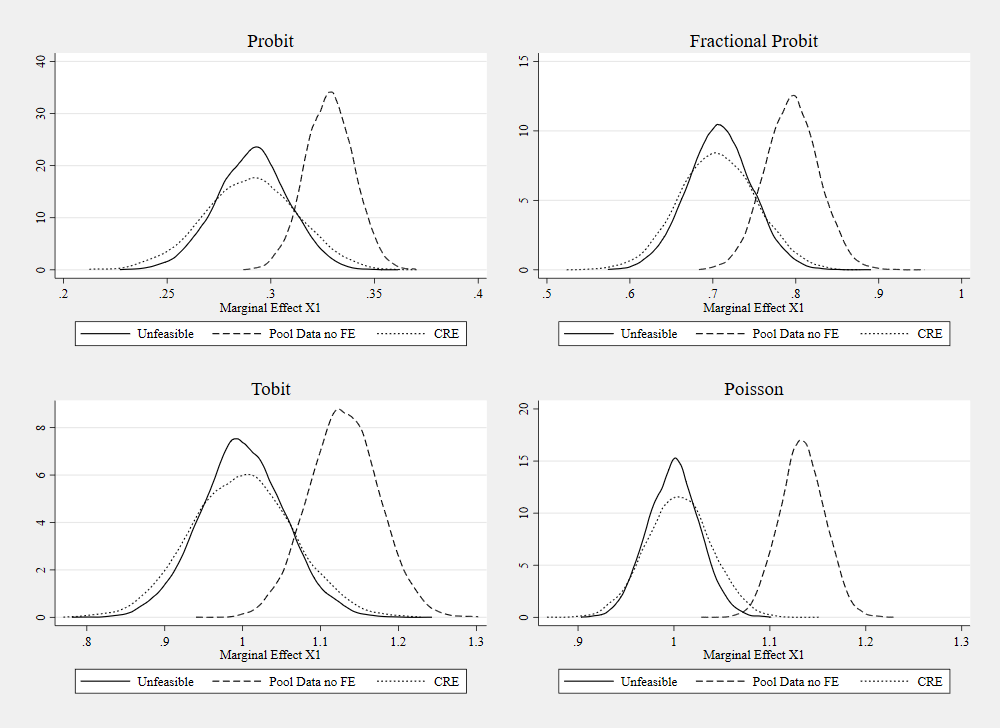
\includegraphics{simulation/fig1.png}

}

\caption{\label{fig-cre}Estimated marginal effects/Coefficient densities
for non-linear models}

\end{figure}%

As expected, controlling for the unobserved effects, the unfeasible
estimator provides what we would consider to be the benchmark/true
estimates of coefficients/marginal effects given the sample and data
generating process. For Table~\ref{tbl-cre}, we use the average
coefficients/marginal effects of the unfeasible estimator to represent
the true point estimate, and use those to construct the bias and mean
absolute error for the other estimators.

Because the individual effects are constructed to be correlated with the
explanatory variables, the estimated coefficients are biased when they
are ignored, and coefficients are estimated using pooled estimators. The
magnitude of the bias is approximately 12-13\% with respect to the point
estimate of the coefficient or marginal effect.

On the other hand, the CRE approach seems to provide consistent
estimates for the coefficients/marginal effects, with a distribution
that is centered around the true point estimate, with slightly higher
variance than the benchmark. Based on the results from
Table~\ref{tbl-cre}, the bias of the CRE approach is negligible, with a
MAE that is about 20\% to 30\% larger than the benchmark.

\begin{longtable}[]{@{}
  >{\raggedright\arraybackslash}p{(\columnwidth - 8\tabcolsep) * \real{0.2000}}
  >{\centering\arraybackslash}p{(\columnwidth - 8\tabcolsep) * \real{0.2000}}
  >{\centering\arraybackslash}p{(\columnwidth - 8\tabcolsep) * \real{0.2000}}
  >{\centering\arraybackslash}p{(\columnwidth - 8\tabcolsep) * \real{0.2000}}
  >{\centering\arraybackslash}p{(\columnwidth - 8\tabcolsep) * \real{0.2000}}@{}}
\caption{Bias and MAE for the estimated marginal effects/Coefficients
for non-linear models}\label{tbl-cre}\tabularnewline
\toprule\noalign{}
\begin{minipage}[b]{\linewidth}\raggedright
\end{minipage} & \begin{minipage}[b]{\linewidth}\centering
Probit
\end{minipage} & \begin{minipage}[b]{\linewidth}\centering
FProbit
\end{minipage} & \begin{minipage}[b]{\linewidth}\centering
Tobit
\end{minipage} & \begin{minipage}[b]{\linewidth}\centering
Poisson
\end{minipage} \\
\midrule\noalign{}
\endfirsthead
\toprule\noalign{}
\begin{minipage}[b]{\linewidth}\raggedright
\end{minipage} & \begin{minipage}[b]{\linewidth}\centering
Probit
\end{minipage} & \begin{minipage}[b]{\linewidth}\centering
FProbit
\end{minipage} & \begin{minipage}[b]{\linewidth}\centering
Tobit
\end{minipage} & \begin{minipage}[b]{\linewidth}\centering
Poisson
\end{minipage} \\
\midrule\noalign{}
\endhead
\bottomrule\noalign{}
\endlastfoot
True:Bias & -0.000 & -0.000 & -0.000 & -0.000 \\
True:MAE & 0.014 & 0.031 & 0.043 & 0.022 \\
Pool:Bias & 0.037 & 0.087 & 0.130 & 0.134 \\
Pool:MAE & 0.037 & 0.087 & 0.130 & 0.134 \\
CRE:Bias & -0.001 & -0.002 & -0.001 & 0.005 \\
CRE:MAE & 0.018 & 0.037 & 0.052 & 0.027 \\
\emph{N} & 10000 & 10000 & 10000 & 10000 \\
\end{longtable}

\section{Conclusion}\label{sec-5}

This paper introduces the \texttt{cre} command, a prefix-type command
that facilitates the implementation of Correlated Random Effects (CRE)
models with a wide range of official and user-written Stata estimation
commands. The CRE approach offers a middle ground between fixed effects
and random effects models, addressing some of their limitations,
particularly in the context of nonlinear model estimation.

As previously discussed in the literature, our Monte Carlo simulations
show that the CRE approach, implemented through the \texttt{cre}
command, consistently estimates coefficients and marginal effects,
performing comparably to the unfeasible estimators that directly control
for unobserved factors. The simulations reveal negligible bias, with an
increase in the variance of the estimates, which is consistent with
theoretical expectations.

The \texttt{cre} command addresses a significant gap in Stata's
econometric toolkit, providing a user-friendly implementation of CRE
models. This tool may prove valuable for researchers working with panel
data or nested data structures, where standard fixed effects approaches
may be challenging or nonexistent, and random effects assumptions are
not appropriate.

\section{Acknowledgments}\label{acknowledgments}

Thanks to Aashima Sinha for her help in the preparation and comments for
this paper, and Enrique Pinzon for his encouragement on pushing this
project forward.

\clearpage

\bibliographystyle{sj}
\bibliography{references.bib}


\begin{aboutauthors}

Fernando Rios-Avila is a research scholar at the Levy Economics
Institute of Bard College under the Distribution of Income and Wealth
program. His research interests include applied econometrics, labor
economics, and poverty and inequality. He has contributed many commands
to Statistical Software Components and written articles for the Stata
Journal.

\end{aboutauthors}

\end{document}
